\documentclass{beamer}

\input{../../src/common/base_header.tex}
\input{../../src/common/themes/theme_choice_light.tex}
\input{../../src/common/themes/theme.tex}
\input{../../src/common/math/base.tex}
\input{../../src/common/math/advanced.tex}
\input{../../src/common/environments/base.tex}
\input{../../src/common/tikz/base.tex}
\input{../../src/common/themes/more_colours.tex}
\input{../../src/common/algorithms/base.tex}
\input{../../src/common/algorithms/advanced.tex}
\input{../../src/common/language/julia.tex}





\usetheme{Madrid}

\title{Comparaison de formulations du problème du voyageur de commerce}
\author{Ivan Lejeune}
\date{\today}

\begin{document}

% =========================
\frame{\titlepage}

% =========================
\begin{frame}{Introduction}
\begin{itemize}
    \item Problème du voyageur de commerce (TSP)
    \item Trouver le plus court cycle hamiltonien
    \item Problème NP-difficile
    \item Objectif: comparer différentes formulations MILP
\end{itemize}
\end{frame}

% =========================
\begin{frame}{Définition du problème}
\begin{itemize}
    \item Graphe complet avec distances $c_{ij}$
    \item Variables:
    \[
    x_{ij} =
    \begin{cases}
    1 & \text{si l'arc est utilisé} \\
    0 & \text{sinon}
    \end{cases}
    \]
    \item Contraintes:
    \begin{itemize}
        \item Une entrée par sommet
        \item Une sortie par sommet
    \end{itemize}
\end{itemize}
\end{frame}

% =========================
\begin{frame}{Formulation MTZ}
\begin{itemize}
    \item Variables supplémentaires: $y_i$
    \item Interprétation: ordre de visite
    \item Élimination des sous-tours
\end{itemize}

\[
x_{ij}(n-1) + y_i - y_j \leq n-2
\]

\begin{itemize}
    \item Formulation compacte
    \item Relaxation linéaire faible
\end{itemize}
\end{frame}

% =========================
\begin{frame}{Formulation SF}
\begin{itemize}
    \item Variables: $q_{ij}$ (flux)
    \item Idée: envoyer $n-1$ unités depuis le sommet 1
    \item Chaque sommet consomme 1 unité
\end{itemize}

\begin{itemize}
    \item Assure la connectivité globale
    \item Relaxation plus forte
\end{itemize}
\end{frame}

% =========================
\begin{frame}{Programme linéaire --- MTZ}
    \begin{equation*}
        MTZ = 
        \begin{cases}
            \min z = \sum_{i=1}^n \sum_{j=1}^n c_{ij} x_{ij} \\
            \sum_{i,j} x_{ij} = 1 \quad \forall i \in \{1, \ldots, n\} \\
            \sum_{i,j} x_{ij} = 1 \quad \forall j \in \{1, \ldots, n\} \\
            x_{ij} (n-1) + y_i - y_j \leq n-2 \quad \forall i,j \in \{1, \ldots, n\}, i \neq j \\
            x_{ij} \in \{0,1\} \quad \forall i,j \in \{1, \ldots, n\} \\
            y_i \geq 0 \quad \forall i \in \{1, \ldots, n\}
        \end{cases}
    \end{equation*}
\end{frame}

% =========================
\begin{frame}{Programme linéaire --- SF}
    \begin{equation*}
        SF = 
		\begin{cases}
			\min z = \sum_{i=1}^n \sum_{j=1}^n c_{ij} x_{ij} \\
			\sum_{i,j} x_{ij} = 1 \quad \forall i \in \{1, \ldots, n\} \\
			\sum_{i,j} x_{ij} = 1 \quad \forall j \in \{1, \ldots, n\} \\
			q_{ij} \leq (n-1) x_{ij} \quad \forall i,j \in \{1, \ldots, n\}, i \neq j \\
			\sum_{j=1}^n q_{1j} = n-1 \\
			\sum_{i\neq j} q_{ji} - \sum_{i\neq j} q_{ij} = 1 \quad \forall j \in \{2, \ldots, n\} \\
			x_{ij} \in \{0,1\} \quad \forall i,j \in \{1, \ldots, n\} \\
			0 \leq q_{ij} \leq n-1 \quad \forall i,j \in \{1, \ldots, n\}
		\end{cases}
    \end{equation*}
\end{frame}


% =========================
\begin{frame}{Comparaison théorique}
\begin{center}
\begin{tabular}{c|c}
MTZ & SF \\
\hline
Simple & Plus complexe \\
Peu de variables & Plus de variables \\
Relaxation faible & Relaxation forte \\
\end{tabular}
\end{center}

\bigskip

\textbf{Conclusion:} SF devrait être plus performante
\end{frame}

% =========================
\begin{frame}{Implémentation}
\begin{itemize}
    \item Langage: Julia
    \item Librairie: JuMP + Cbc
    \item Parsing des instances à partir des tableaux de distances
    \item Implémentation modulaire:
    \begin{itemize}
        \item solve\_mtz
        \item solve\_sf
    \end{itemize}
\end{itemize}
\end{frame}

% =========================
\begin{frame}{Le code MTZ - 1}
    \juliaFile{generic_mtz_import_1.jl}
\end{frame}

% =========================
\begin{frame}{Le code MTZ - 2}
    \juliaFile{generic_mtz_import_2.jl}
\end{frame}

% =========================
\begin{frame}{Le code SF - 1}
    \juliaFile{generic_sf_import_1.jl}
\end{frame}

% =========================
\begin{frame}{Le code SF - 2}
    \juliaFile{generic_sf_import_2.jl}
\end{frame}

% =========================
\begin{frame}{Relaxations linéaires}
\begin{itemize}
    \item Calcul des relaxations pour plusieurs instances
    \item Observation:
    \begin{itemize}
        \item SF donne des bornes plus élevées
        \item Relaxation plus serrée
    \end{itemize}
\end{itemize}

\textbf{Impact:} meilleure efficacité du branch-and-bound
\end{frame}

% =========================
\begin{frame}{Résultats expérimentaux --- 1}
\begin{itemize}
    \item Comparaison des temps de calcul
    \item Comparaison des solutions obtenues
\end{itemize}

\begin{center}
    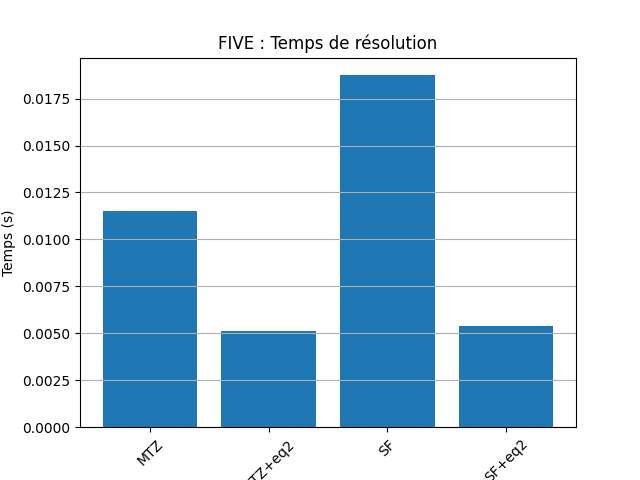
\includegraphics[width=0.7\textwidth]{FIVE_time.png}
\end{center}

\end{frame}

% =========================
\begin{frame}{Résultats expérimentaux --- 2}

\begin{center}
    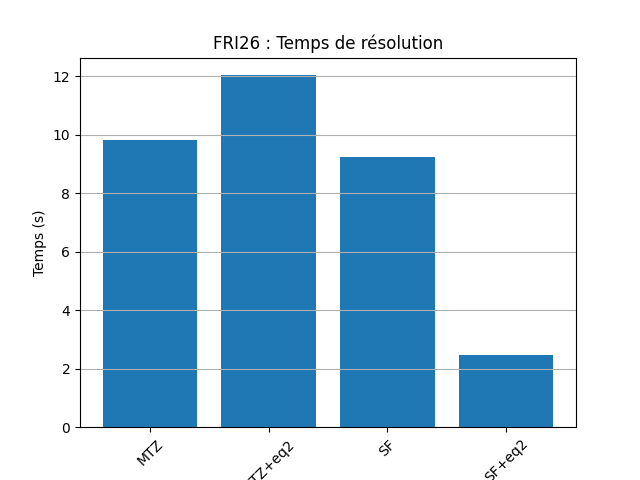
\includegraphics[width=0.7\textwidth]{FRI26_time.png}
\end{center}

\end{frame}

% =========================
\begin{frame}{Résultats expérimentaux --- 3}

\begin{center}
    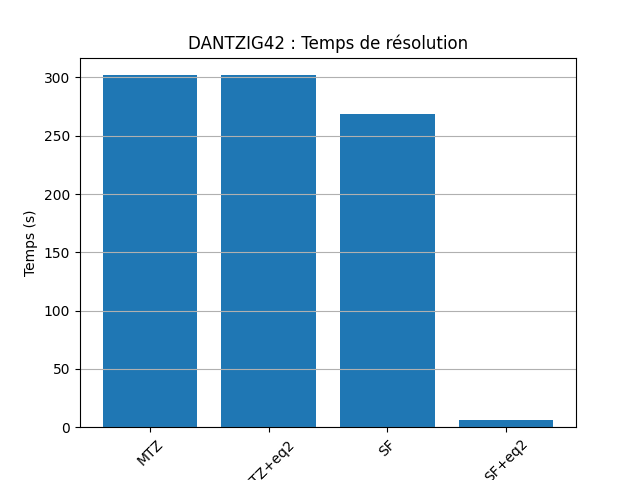
\includegraphics[width=0.7\textwidth]{DANTZIG42_time.png}
\end{center}

\end{frame}

% =========================
\begin{frame}{Résultats expérimentaux --- 4}

\begin{center}
    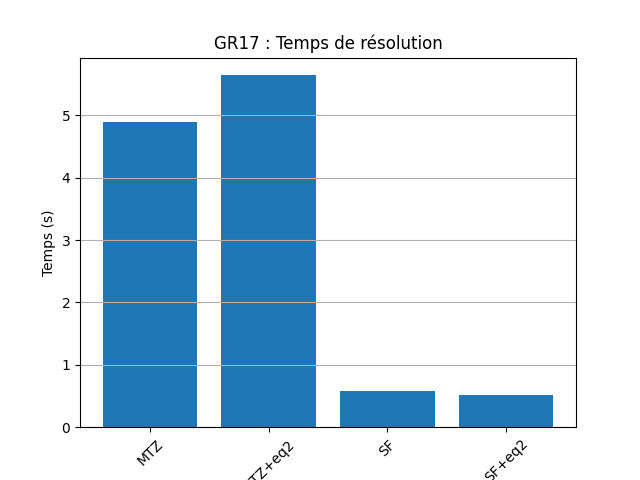
\includegraphics[width=0.7\textwidth]{GR17_time.png}
\end{center}

\end{frame}

% =========================
\begin{frame}{Synthèse des résultats}
\begin{itemize}
    \item SF plus rapide que MTZ sauf sur les plus petites instances
    \item Écart de temps plus important sur certaines instances
    \item Importance de la relaxation linéaire
\end{itemize}

\end{frame}

% =========================
\begin{frame}{Ajout de l'inégalité $x_{ij} + x_{ji} \leq 1$}
\begin{itemize}
    \item Élimine les arcs bidirectionnels
    \item Réduit les solutions fractionnaires
    \item Améliore la relaxation
\end{itemize}

\textbf{Résultat:} amélioration des performances
\end{frame}

% =========================
\begin{frame}{Test sur ATT48}
\begin{itemize}
    \item Instance plus grande
    \item Étude de la convergence en temps
\end{itemize}

\begin{center}
    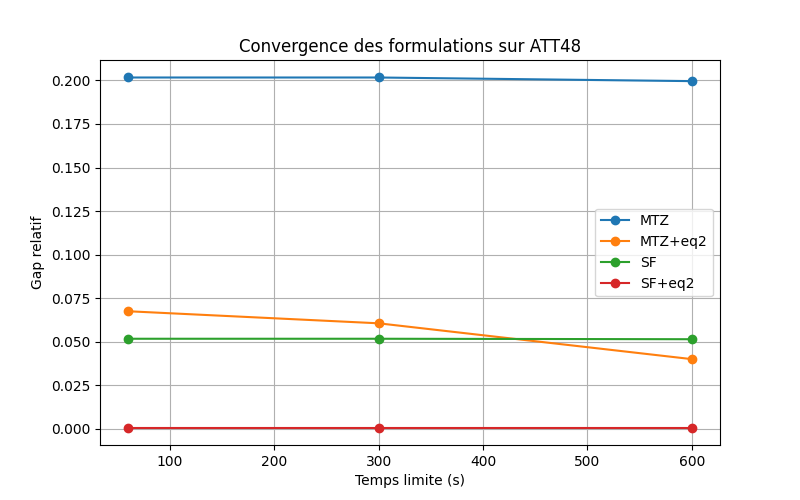
\includegraphics[width=0.7\textwidth]{att48_gap.png}
\end{center}

\end{frame}

% =========================
\begin{frame}{Difficultés rencontrées}
\begin{itemize}
    \item Modélisation MTZ (le problème de l'infaisabilité)
    \item Parsing des données
    \item Temps de calcul
    \item Compréhension des relaxations
\end{itemize}
\end{frame}

% =========================
\begin{frame}{Conclusion}
\begin{itemize}
    \item SF plus performante que MTZ
    \item La relaxation linéaire est un facteur clé
    \item Le rajout de contraintes supplémentaires améliore les performances
\end{itemize}

\bigskip

\textbf{Ouverture:}
\begin{itemize}
    \item Autres formulations (DFJ)
    \item Rajout de contraintes généralisées
\end{itemize}
\end{frame}

% =========================
\begin{frame}{Questions}
\centering
\Huge Questions?
\end{frame}

\end{document}